\subsection{NGTNs and User Defined Conductors}

The use of user defined conductors (UDC) has been implemented in order to better
represent the heat flow from the spacers, the ICs and the antenna. The further use of GLs
might be studied in further iterations.

\subsubsection{Non-Geometrical Thermal Nodes}
As has been mentioned in the previous subsection, the use of Non-Geometrical Thermal Nodes to represent
the ICs in each stack PCB relies in the definition of GLs from said nodes to the nodes of the PCB mesh.
Therefore, for each IC, depending on its package, a value of conductance has been set.

\paragraph{}

These values have been extracted from similar ICs empirical resistance due to the lack of junction to case resistance information.
Also, as this measure is defined only to compare between ICs and doesn't provide any standalone value,
it has been further seen fit to extract the values in this manner. Do note that the values taken are order of magnitude
aproximations.

\paragraph{}

A list of the conductances for NGTNs is provided next:

\begin{table}[H]
    \centering
    \begin{tabular}{@{}ccccc@{}}
    \toprule
    \textbf{ESATAN Name} & \textbf{Component} & \textbf{Package} & $\mathbf{\Theta_{JB} (K/W)}$ & \textbf{G (W/K)} \\ \midrule
    NGTN\_ADCS\_U1       & LPV542             & X1SON            & 20                           & 0.05             \\
    NGTN\_ADCS\_U2       & LPV542             & X1SON            & 20                           & 0.05             \\
    NGTN\_ADCS\_U3       & LPV542             & X1SON            & 20                           & 0.05             \\
    NGTN\_ADCS\_U4       & IIM-42652          & 14-pin LGA       & 15                           & 0.07             \\
    NGTN\_ADCS\_U5       & BD2606MVV          & SQFN016V4040     & 5                            & 0.20             \\
    NGTN\_ADCS\_U6       & TMUX1108RSVR       & RSV (QFN, 16)    & 5                            & 0.20             \\
    NGTN\_ADCS\_U7       & MMC5983MA          & ILSP             & 15                           & 0.07             \\
    NGTN\_Batt\_Heater   & x                  & x                & x                            & x                \\
    NGTN\_EPS\_IC1       & DS2782E+           & TDFN-10          & 10                           & 0.10             \\
    NGTN\_EPS\_IC2       & ISL9120IRTNZ       & TQFN             & 10                           & 0.10             \\
    NGTN\_EPS\_U1        & SPV1040TTR         & TSSOP8           & 15                           & 0.07             \\
    NGTN\_EPS\_U2        & SPV1040TTR         & TSSOP8           & 15                           & 0.07             \\
    NGTN\_EPS\_U3        & SPV1040TTR         & TSSOP8           & 15                           & 0.07             \\
    NGTN\_EPS\_U4        & LTC4040EUFD\#PBF   & QFN              & 5                            & 0.20             \\
    NGTN\_OBC\_STM32     & STM32L476RGTx      & LQFP - 64 pins   & 10                           & 0.10             \\
    NGTN\_OBC\_SX1262    & SX1262IMLTRT       & QFN (24L)        & 5                            & 0.20             \\
    NGTN\_PLTOP\_U1      & HMC342LC4          & SMT              & 5                            & 0.20             \\
    NGTN\_PLTOP\_U2      & HMC516LC5          & SMT              & 5                            & 0.20             \\
    NGTN\_PLTOP\_Y1      & HMC506LP4ETR       & QFN Leadless SMT & 5                            & 0.20             \\
    NGTN\_PLUNDER\_U1    & CMD271P3           & QFN Package      & 5                            & 0.20             \\
    NGTN\_PLUNDER\_U2    & SIM-14+            & HV1195           & 5                            & 0.20             \\
    NGTN\_PLUNDER\_U3    & LT5537EDDB\#TRMPBF & DFN (8L)         & 10                           & 0.10             \\
    NGTN\_PLUNDER\_U4    & LEE2-6+            & MC1630-1 (6L)    & 15                           & 0.07             \\
    NGTN\_PLUNDER\_U5    & LEE2-6+            & MC1630-1 (6L)    & 15                           & 0.07             \\
    NGTN\_PLUNDER\_U7    & HMC358MS8GE        & MSOP8G SMT       & 15                           & 0.07             \\ \bottomrule
    \end{tabular}
    \caption{NGTNs UDC assigned values.}
\end{table}

\subsubsection{Spacers}

Due to the lack of the modelling of holes in the PCBs, it is to be expected that the top to bottom conductivity
of the PCB stack is reduced. In order to mitigate this effect, user defined conductors have been placed between each one
of the spacers of the stack, with the conductance set to that of stainless steel. Note that this is a first approximation
and a more detailed mathematical model might be needed to correlate experimental results.

\begin{figure}[H]
    \centering
    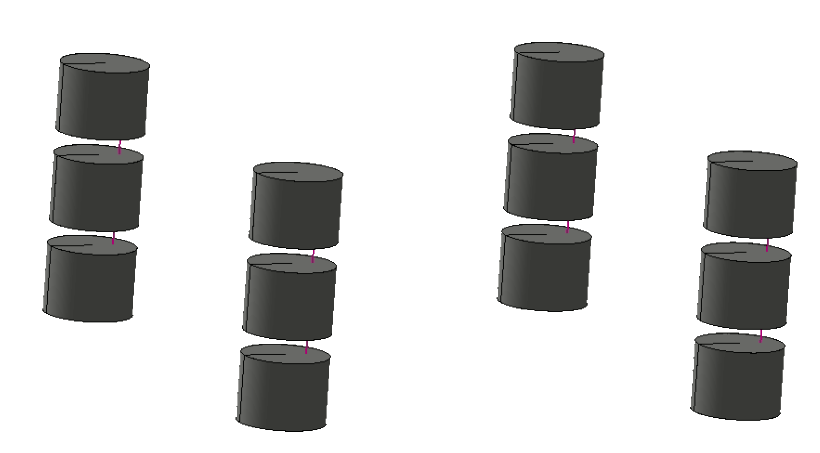
\includegraphics[width=0.5\linewidth]{res/img/5_2_udcs/spacersudcs.PNG}
    \caption{Spacers with GLs between them in ESATAN.}
    \label{fig:spacersudcs}
\end{figure}

\subsubsection{Antenna}

The COMMS antenna is soldered and screwed to the interior surface of a lateral board. The conductance of the conctact
has been modeled as if a square centimeter of the antenna was in contact with the lateral board, with the conductivity of
tin, as it is the material it is soldered and covered with.

\begin{figure}[H]
    \centering
    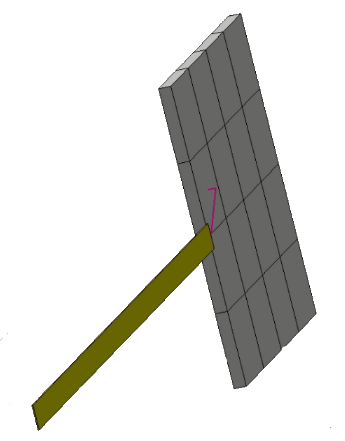
\includegraphics[width=0.3\linewidth]{res/img/5_2_udcs/antennalatudc.PNG}
    \caption{Antenna connected to a lateral board through a UDC in ESATAN.}
    \label{fig:antennaudc}
\end{figure}